\documentclass[xcolor=table]{beamer}
\usepackage{beamerthemesplit}
\usepackage{wrapfig}
\usetheme{SPbGU}
\usepackage{pdfpages}
\usepackage{amsmath}
\usepackage{cmap}
\usepackage[T2A]{fontenc}
\usepackage[utf8]{inputenc}
\usepackage[english]{babel}
\usepackage{indentfirst}
\usepackage{mathtools}
\usepackage{tikz}
\usepackage{multirow}
\usepackage[noend]{algpseudocode}
\usepackage{algorithm}
\usepackage{algorithmicx}
\usepackage{fancyvrb}
\usetikzlibrary{calc}
\usetikzlibrary{shapes,arrows}
\usetikzlibrary{arrows,automata}
\usetikzlibrary{positioning}

\usepackage{fontawesome}

\usetikzlibrary{shapes.callouts}

\usepackage{xparse}

%for [[ ]]
\usepackage{stmaryrd}


\tikzset{
    invisible/.style={opacity=0,text opacity=0},
    visible on/.style={alt=#1{}{invisible}},
    alt/.code args={<#1>#2#3}{%
      \alt<#1>{\pgfkeysalso{#2}}{\pgfkeysalso{#3}} % \pgfkeysalso doesn't change the path
    },
}

\NewDocumentCommand{\mycallout}{r<> O{opacity=0.8,text opacity=1} m m}{%
\tikz[remember picture, overlay]\node[align=center, fill=cyan!20, text width=3.5cm,
#2,visible on=<#1>, rounded corners,
draw,rectangle callout,anchor=pointer,callout relative pointer={(230:1cm)}]
at (#3) {#4};
}

%\newcommand{\tikzmark}[1]{\tikz[overlay,remember picture,baseline=-0.5ex] \node (#1) {};}



\usepackage{tabularx}
\newcolumntype{Y}{>{\raggedleft\arraybackslash}X}

\renewcommand{\thealgorithm}{}

\newtheorem{mytheorem}{Theorem}
\renewcommand{\thealgorithm}{}

\newcommand{\tikzmark}[1]{\tikz[overlay,remember picture] \node (#1) {};}
\def\Put(#1,#2)#3{\leavevmode\makebox(0,0){\put(#1,#2){#3}}}

\newcommand{\ltz}{$< 1$}


\tikzset{
    state/.style={
           rectangle,
           rounded corners,
           draw=black, very thick,
           minimum height=2em,
           inner sep=2pt,
           text centered,
           },
}

\beamertemplatenavigationsymbolsempty

\title[Partial Evaluation for GPGPU]{POSTER: Optimizing GPU Programs by Partial Evaluation}
%\subtitle[YaccConstructor]{Parsing techniques for graph analysis}
% То, что в квадратных скобках, отображается в левом нижнем углу.
\institute[JB Research, SPbSU]{
JetBrains Research, Programming Languages and Tools Lab  \\
Saint Petersburg University
}

% То, что в квадратных скобках, отображается в левом нижнем углу.
\author[Semyon Grigorev]{Aleksey Tyurin, Daniil Berezun, \textbf{Semyon Grigorev}}

\date{February 24, 2020}

\begin{document}
{
\begin{frame}[fragile]
  \begin{table}
  \centering
  \begin{tabularx}{\linewidth}{YcX}
    
\includegraphics[height=1.5cm]{pictures/jetbrainsResearch.pdf} \hfill
    & \begin{minipage}[t]{0.3\textwidth}\center \vspace{-1cm}  PPoPP 2020
      \end{minipage}
    & \hfill 
\includegraphics[height=1.5cm]{pictures/SPbGU_Logo.png}
  \end{tabularx}
  \end{table}
  \titlepage
\end{frame}
}

\begin{frame} \frametitle{GPGPU Architecture}
  \begin{minipage}[m]{0.4\linewidth}
  \raisebox{-0.5\totalheight}{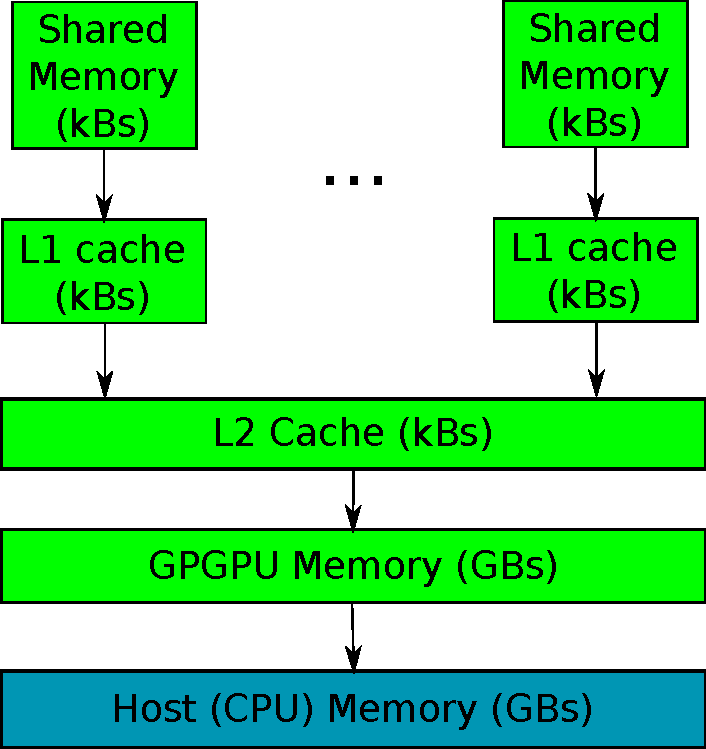
\includegraphics[width=\textwidth]{pictures/GPUMemory2.pdf}}
  \end{minipage}\hfill
  \begin{minipage}[m]{0.55\linewidth}
  GPGPU memory hierarchy
  \pause
  \begin{itemize}
        \item Global memory
        \begin{itemize}
          \item[\faSmileO] Big
          \item[\faFrownO] Slow
        \end{itemize}
        \pause
        \item Shared memory
          \begin{itemize}
            \item[\faSmileO] Fast
            \item[\faFrownO] Relatively small
            \item[\faFrownO] Manual allocation mamagement
          \end{itemize}
          \pause
          \item Constant memory
          \begin{itemize}
            \item[\faSmileO] Fast
            \begin{itemize}
              \item[\faFrownO] Only for appropriate access pattern
            \end{itemize}
            \item[\faFrownO] Small
            \item[\faFrownO] Static allocation
          \end{itemize}
          \pause
        \item \textbf{Memory traffic is a bottleneck}
  \end{itemize}

  \end{minipage}

  \end{frame}


  \begin{frame}[fragile] \frametitle{Data Processing}
    \begin{itemize}
      \item Substring matching
      \item 2D convolution
      \item Filtering by using Hidden Markov Models (HMM)
    \end{itemize}
    \pause
    \tikzmark{zzz}{
    }
    \begin{verbatim}
      __global__ void handleData
                         (int* filterParams, int* data, ...)
      {
         __shared__ int cachedFilterParams[size];

         /*some code to load filterParams
           to cachedFilterParams*/
         ...
      }
    \end{verbatim}
    \pause
    \onslide<3>{\tikz[overlay,remember picture]{\draw[draw=red, fill opacity=0.2, line width=0.25mm] ($ (zzz) + (5.15,-0.8)$) rectangle ($  (zzz) + (8.6,-1.3)$);}}
    \onslide<4>{\tikz[overlay,remember picture]{\draw[draw=red, fill opacity=0.2, line width=0.25mm] ($ (zzz) + (8.9,-0.8)$) rectangle ($  (zzz) + (10.8,-1.3)$);}}
    \onslide<5>{\tikz[overlay,remember picture]{\draw[draw=red, fill opacity=0.2, line width=0.25mm] ($ (zzz) + (1.5,-1.8)$) rectangle ($  (zzz) + (10,-3.7)$);}}
  \end{frame}


  \begin{frame}[fragile] \frametitle{Big Data Processing}
    \begin{itemize}
      \item Substring matching $\Rightarrow$ Data curving (cyber forensics)
      \item 2D convolution $\Rightarrow$ Image processing
      \item Filtering by using HMMs  $\Rightarrow$ Homology search (bioinformatics)
    \end{itemize}
    \pause

    \tikzmark{xxx}{
    }
    \begin{verbatim}
      __global__ void handleData
                         (int* filterParams, int* data, ...)
      {
         ...
      }
    \end{verbatim}
    \pause
    \onslide<4-6>{\tikz[overlay,remember picture]{\draw[draw=red, fill opacity=0.2, line width=0.25mm] ($ (xxx) + (5.15,-0.8)$) rectangle ($  (xxx) + (8.6,-1.3)$);}
    \mycallout<4-6>[opacity=1]{$ (xxx) + (5.15,-0.8)$}{One filter for many data chunks}
    }
    \onslide<3-6>{\tikz[overlay,remember picture]{\draw[draw=red, fill opacity=0.2, line width=0.25mm] ($ (xxx) + (8.9,-0.8)$) rectangle ($  (xxx) + (10.8,-1.3)$);}
    \mycallout<3-6>[opacity=1]{$ (xxx) + (8.9,-0.8)$}{Many data chunks $\Rightarrow$ many procedure runs}
    }
    \vspace{-1cm}
\begin{center}
    \onslide<5-6>{\texttt{filterParams} is static during one data processing session\\}
    \vspace{0.5cm}
    \onslide<6>{How can we use this fact to optimize our procedure?}
\end{center}
  \end{frame}

\begin{frame}[fragile] \frametitle{Partial Evaluation or Specialization}
   $$\llbracket \underbrace{handleData}_{handleData} \rrbracket [filterParams, data] = \llbracket \underbrace{\llbracket {\overbrace{mix}^{\mathclap{\text{partial evaluator}}}} \rrbracket [handleData,filterParams]}_{handleData_{mix}}\rrbracket [data]$$
  %$\textbf{mix}$ is a partial evaluator \\
  \vspace{-0.3cm}
  \pause
  \begin{minipage}[t]{0.55\textwidth}
   \vspace{0.82cm}
   \tikzmark{xxx}{
   }
  \begin{verbatim}
handleData (filterParams, data)
{
  res = new List()
  for d in data
     for e in filterParams
        if d % e == 0
        then res.Add(d)
  return res
}
  \end{verbatim}
\end{minipage}
~
\begin{minipage}[t]{0.35\textwidth}
  \pause
  \vspace{0.5cm}
  $\llbracket \llbracket mix \rrbracket [handleData,[2;3]]\rrbracket$
  \pause
  \begin{verbatim}
handleData (data)
{
  res = new List()
  for d in data
    if d % 2 == 0 ||
       d % 3 == 0
    then res.Add(d)
  return res
}
  \end{verbatim}
\end{minipage}
\onslide<5>{\tikz[overlay,remember picture]{\draw[draw=red, fill opacity=0.2, line width=0.25mm] ($ (xxx) + (0,-2.3)$) rectangle ($  (xxx) + (11,-3.7)$);}}
\end{frame}

\begin{frame}[fragile] \frametitle{Evaluation Setup}
  \begin{itemize}
    \item We use AnyDSL framework for specialization
    \begin{itemize}
      \item Special DSL which can be specialized and compiled
      \item Ahead-of-time specialization
    \end{itemize}
    \pause
    \item Algorithms
    \begin{itemize}
      \item Na\"{\i}ve multiple substring matching
      \item 2D convolution
    \end{itemize}
    \pause
    \item Environment
    \begin{itemize}
      \item \textbf{GTX-1070}: Pascal architecture, 8GB GDDR5, 1920 CUDA cores
      \item \textbf{Tesla T4}: Turing architecture, 16GB GDDR6, 2560 CUDA cores
    \end{itemize}

  \end{itemize}
\end{frame}


\begin{frame}[fragile] \frametitle{Evaluation: Substring Matching}
  \begin{itemize}
  \item Application: data curving
  \item Subject string: byte sequence from real hard drive
  \item Patterns: 16 file signatures from GCK’s file signatures table\footnote{\url{https://www.garykessler.net/library/file_sigs.html}}
  \end{itemize}
  \begin{center}
  \begin{minipage}[t]{0.48\textwidth}
    \begin{center}
      \tikzmark{x}{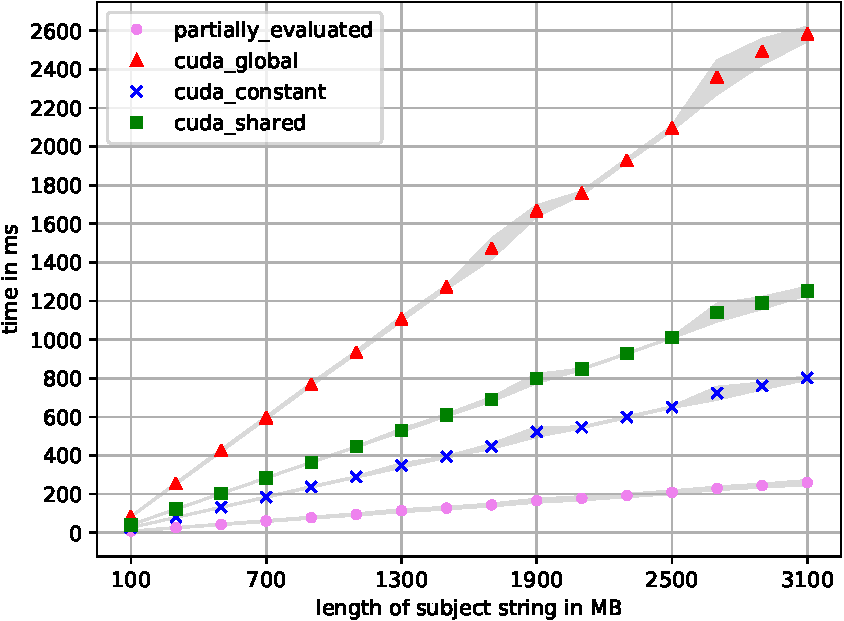
\includegraphics[width=\textwidth]{pictures/Substr_1070-crop}}
  \\Results for GTX-1070
\end{center}
\end{minipage}
\begin{minipage}[t]{0.48\textwidth}
  \begin{center}
{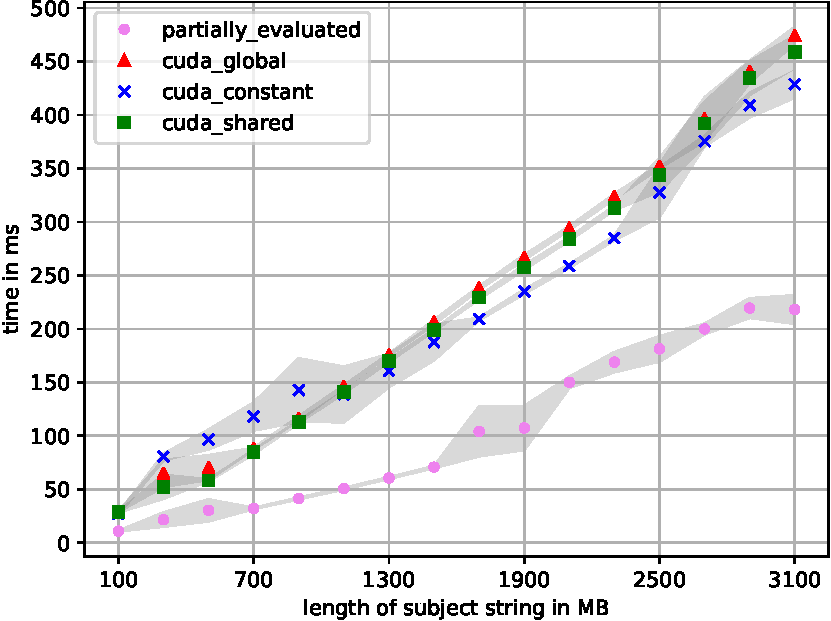
\includegraphics[width=\textwidth]{pictures/Substr_T4-crop}}
\\Results for Tesla T4
\end{center}
\end{minipage}
\end{center}
\onslide<2>{\tikz[overlay,remember picture]{\draw[draw=red, fill opacity=0.2, line width=0.25mm] ($ (x) + (0.8,4.15)$) rectangle ($  (x) + (2.7,3.9)$);}}
\onslide<3>{\tikz[overlay,remember picture]{\draw[draw=red, fill opacity=0.2, line width=0.25mm] ($ (x) + (0.8,3.95)$) rectangle ($  (x) + (2.7,3.7)$);}}
\onslide<4>{\tikz[overlay,remember picture]{\draw[draw=red, fill opacity=0.2, line width=0.25mm] ($ (x) + (0.8,3.75)$) rectangle ($  (x) + (2.7,3.5)$);}}
\onslide<5>{\tikz[overlay,remember picture]{\draw[draw=red, fill opacity=0.2, line width=0.25mm] ($ (x) + (0.8,3.55)$) rectangle ($  (x) + (2.7,3.3)$);}}
\end{frame}


\begin{frame}[fragile] \frametitle{Evaluation: 2D Convolution}
  \begin{itemize}
  \item Application: image processing
  \item Subject image: random image  of size 1GB %(16384 * 16384)
  \item Filters: random square filters with diameter 3 to 255
  \end{itemize}
  \begin{center}
  \begin{minipage}[t]{0.48\textwidth}
    \begin{center}
  \tikzmark{y}{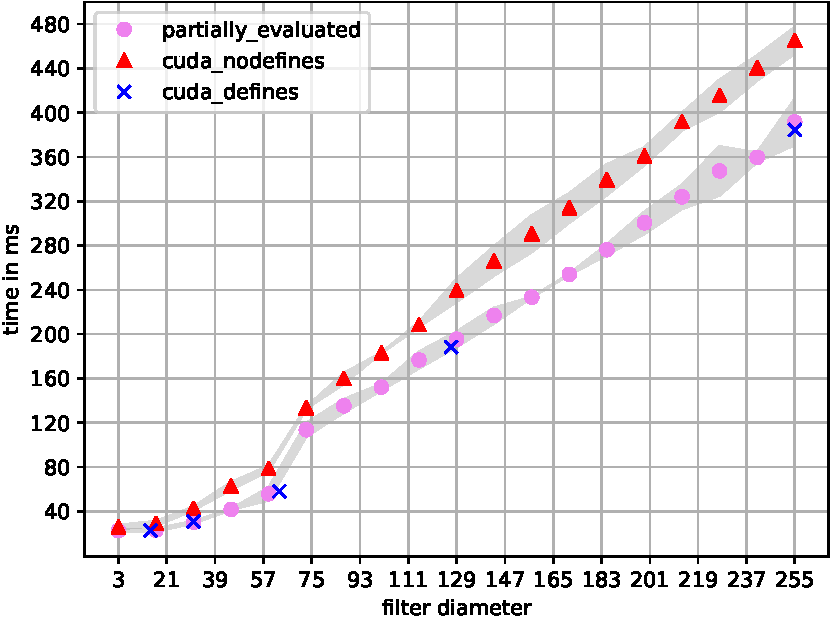
\includegraphics[width=\textwidth]{pictures/Conv_1070-crop}}
  \\Results for GTX-1070
\end{center}
\end{minipage}
\begin{minipage}[t]{0.48\textwidth}
  \begin{center}
{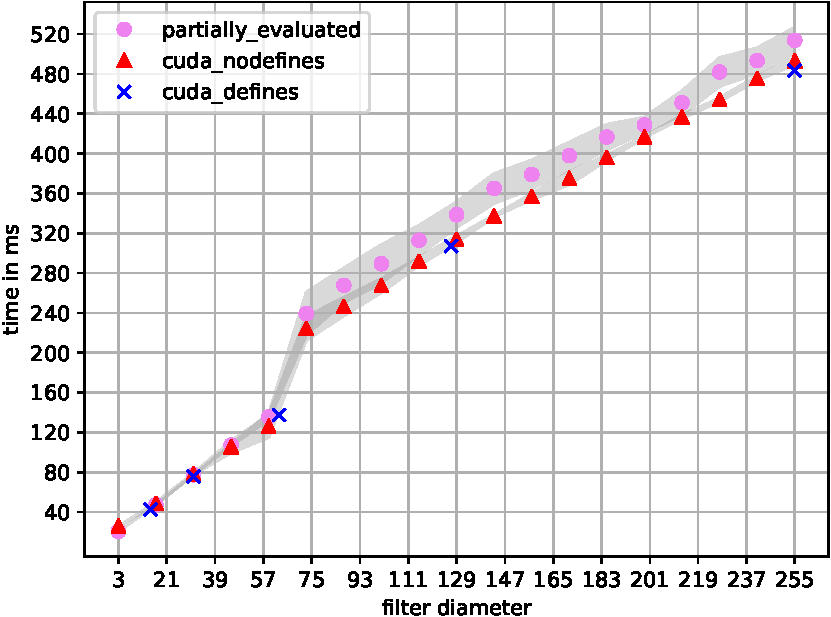
\includegraphics[width=\textwidth]{pictures/Conv_T4-crop}}
\\Results for Tesla T4
\end{center}
\end{minipage}
\end{center}
\onslide<2>{\tikz[overlay,remember picture]{\draw[draw=red, fill opacity=0.2, line width=0.25mm] ($ (x) + (0.7,4.1)$) rectangle ($  (x) + (2.6,3.85)$);}}
\onslide<3>{\tikz[overlay,remember picture]{\draw[draw=red, fill opacity=0.2, line width=0.25mm] ($ (x) + (0.7,3.9)$) rectangle ($  (x) + (2.6,3.65)$);}}
\onslide<4>{\tikz[overlay,remember picture]{\draw[draw=red, fill opacity=0.2, line width=0.25mm] ($ (x) + (0.7,3.7)$) rectangle ($  (x) + (2.6,3.45)$);}}
\end{frame}

\begin{frame} \frametitle{Conclusion}
  \begin{itemize}
   \item Partial evaluation improves performance of GPGPU procedures
   \begin{itemize}
    \item Effect depends on GPU architecture
    \begin{itemize}
      \item Dependencies should be carefully analyzed
    \end{itemize}
    \item Effect depends on the initial memory access pattern
    \begin{itemize}
      \item Irregular pattern --- better performance improvement
    \end{itemize}
   \end{itemize}
  \end{itemize}
\end{frame}

\begin{frame}[fragile] \frametitle{Future Research}
  \begin{itemize}
    \item Migration to CUDA C partial evaluator
    \begin{itemize}
      \item LLVM.mix: partial evaluator for LLVM IR
    \end{itemize}
    \pause
    \item Reduction of specialization overhead
    \begin{itemize}
      \item To be applicable in run-time
    \end{itemize}
    \pause
    \item Integration with shared memory register spilling
    \begin{itemize}
      \item ``RegDem: Increasing GPU Performance via Shared Memory Register Spilling'' (Putt Sakdhnagool et.al. 2019)
    \end{itemize}
    \pause
    \item Evaluation on real-world examples
    \begin{itemize}
      \item Homology search in bioinformatics
      \item Regular expression matching for traffic analysis, log processing
      \item Graph database querying
      \item Ray tracing, path tracing
    \end{itemize}
  \end{itemize}
\end{frame}

\begin{frame}
\frametitle{Contact Information}
\begin{itemize}
  \item Semyon Grigorev:
    \begin{itemize}
      \item \href{mailto:s.v.grigoriev@spbu.ru}{s.v.grigoriev@spbu.ru}
      \item \href{mailto:Semen.Grigorev@jetbrains.com}{Semen.Grigorev@jetbrains.com}
    \end{itemize}

  \item Aleksey Tyurin: \href{mailto:alekseytyurinspb@gmail.com}{alekseytyurinspb@gmail.com}
  \item Daniil Berezun: \href{mailto:daniil.berezun@jetbrains.com}{daniil.berezun@jetbrains.com}

\vspace{0.5cm}
  %\item Dataset and algorithm implementations: \href{https://github.com/SokolovYaroslav/CFPQ-on-GPGPU}{https://github.com/SokolovYaroslav/CFPQ-on-GPGPU}
\end{itemize}
\vspace{0.1cm}
\center{\huge{Thanks!}}
\end{frame}
\end{document}
